\documentclass[../../Main/Main.tex]{subfiles}

\begin{document}
\chapter{Some exactly solvable models of phase transitions}

\section{\emph{1-dim} Ising model}
In this section, we arrive at the exact solution of the one dimensional Ising model.
 There are two techniques for solving the model:
\begin{enumerate}
\item the \emph{recursive method};
\item the \emph{transfer matrix method}.
\end{enumerate}

\subsection{Recursive method}

\subsubsection{Case with \( H=0 \) and free boundary conditions}

\begin{figure}[h!]
\centering
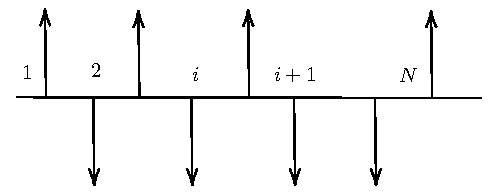
\includegraphics[width=0.5\textwidth]{./img/2__1.pdf}
\caption{\label{fig:6_2} One dimensional Bravais Lattice.}
\end{figure}

Let us consider a Bravais lattice in the one dimensional case, that is just a one dimensional lattice, as in Figure \ref{fig:6_2}.

The canonical partition function of such a system is:
\begin{equation}
  Z_N (T) = \sum_{S_1 = \pm 1}^{} \sum_{S_2 = \pm 1}^{} \dots  \sum_{S_N = \pm 1}^{} \exp [
  \overbrace{ \beta J}^{K}  \sum_{i=1}^{N-1} S_i S_{i+1}  ]
\end{equation}
The two body interaction is the sum in all the neighbours that in that case are \( (i-1) \)  and \( (i+1) \), but we have only to consider the one after, because the one behind is yet taken by the behind site.

We want to solve this partition function. If we consider \emph{free boundary} condition, the \emph{N} does not have a \emph{N+1}, almost for the moment.
Let us define
\begin{equation}
   K \equiv \beta J,  \quad h \equiv \beta H
\end{equation}
Making explicit the sum in the exponential:
\begin{equation*}
  Z_{N} (K) =   \sum_{S_1 = \pm 1}^{} \sum_{S_2 = \pm 1}^{} \dots  \sum_{S_N = \pm 1}^{} e^{K (S_1 S_2 + S_2 S_3 + \dots + S_{N-1}S_N)}
\end{equation*}
What does happen if we just add another spin at the end \( S_{N+1} \) ? Which is the partition function with that new spin? We obtain:
\begin{equation*}
  Z_{N+1} (K) =   \sum_{S_{N+1} = \pm 1}^{} \sum_{S_1 = \pm 1}^{} \sum_{S_2 = \pm 1}^{} \dots  \sum_{S_N = \pm 1}^{} e^{K (S_1 S_2 + S_2 S_3 + \dots + S_{N-1}S_N)} \mathcolorbox{green!20}{ e^{K S_N S_{N+1}} }
\end{equation*}
On the other hand, this sum is just involving this term:
\begin{equation*}
   \sum_{S_{N+1} = \pm 1}^{} e^{K S_N S_{N+1}}  = e^{K S_N} + e^{-K S_N} = 2 \cosh (K S_N) = 2 \cosh(K)
\end{equation*}
where the last equivalence derive from the fact that \( \cosh \) is an even function and it does not depend on \( \pm 1 \). Therefore,
\begin{equation*}
  Z_{N+1} (K) = (2 \cosh (K) ) Z_N (K) \quad \text{and} \quad   Z_{N} (K) = (2 \cosh (K)) Z_{N-1} (K)
\end{equation*}
By performing a backward iteration,
\begin{equation*}
  Z_N (K) = Z_1 (2 \cosh(K) )^{N-1}
\end{equation*}
Since \( Z_1 = \sum_{S_1=\pm1}^{} 1 = 2 \),
we have
\begin{empheq}[box=\myyellowbox]{equation}
   Z_N (T) = 2 (2 \cosh(K) )^{N-1}
\end{empheq}
The free energy is
\begin{equation}
  F_N (K) = - k_B T \ln{Z_N (K)} = - k_B T \ln{2} - k_B T (N-1) \ln{\qty(2 \cosh (K))}
\end{equation}
and taking the thermodynamic limit it becomes
\begin{equation}
  f_b (T) \equiv \lim_{N \rightarrow \infty } \frac{1}{N} F_N (K)= -k_B T \ln{\qty( 2 \cosh (\frac{J}{k_B T}))}
\end{equation}
As one can see (Figure \ref{fig:6_3}) \( f_b (T)  \) is an analytic function of \emph{T}, so we have no phase transition  at \( T \neq 0 \).

\begin{figure}[h!]
\centering
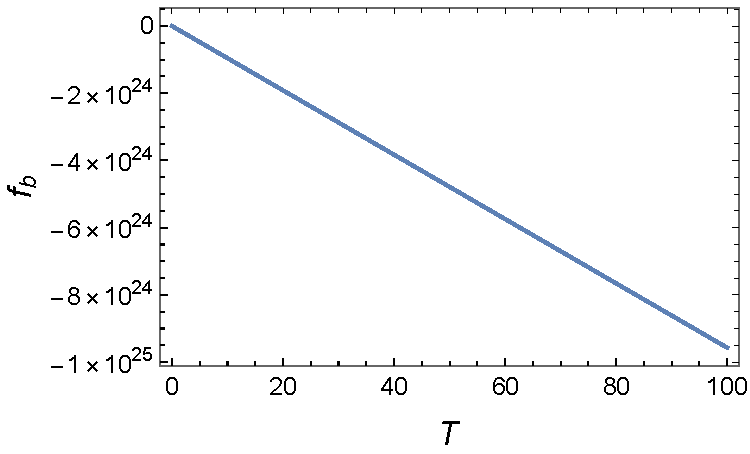
\includegraphics[width=0.7\textwidth]{./img/3__1.pdf}
\caption{\label{fig:6_3} Free energy function in thermodynamic limit for the one dimensional Ising model, for \( k_B = 1.38 \times 10^{23}, J=1\). }
\end{figure}
Now, let us compute the magnetization (the average over the spin \( \expval{S_j}  \)) for a generic site \emph{j} (assume again that \( S_i = \pm 1 \)). This can be done in many ways. Here, we choose one that consider another way to compute \emph{Z} for the \( 1-dim \) Ising model. This method can be useful for other calculations. It is based on the following identity:
\begin{equation}
  \exp [ K S_i S_{i+1}] \underset{(proof)}{=}  \cosh ( K) + S_i S_{i+1} \sinh (K) = \cosh (K) [1+ S_i S_{i+1} \tanh (K)]
  \label{eq:6_5}
\end{equation}
\begin{proof}[Proof of identity \eqref{eq:6_5}]
Remind that 
\begin{equation*}
\cosh x = \frac{e^x + e ^{-x} }{2}, \qquad \sinh x = \frac{e^x - e ^{-x} }{2}
\end{equation*}
Hence, 
\begin{equation*}
    e^x = \cosh{x} + \sinh{x}
\end{equation*}
In our case, 
\begin{equation*}
 e^{k S_i S_{i+1}} = \cosh (K S_i S_{i+1}) +     \sinh (K S_i S_{i+1})
 = \cosh K + S_i S_{i+1} \sinh K 
\end{equation*}
where the last step was obtained considering that \( \cosh \) is an even function, while \( \sinh \) is an odd one.
\end{proof}
Using identity \eqref{eq:6_5}, we obtain
\begin{equation*}
  Z_N (K) = \sum_{\{ S \}  }^{}    \exp [K  \sum_{i=1}^{N-1} S_i S_{i+1}  ] = \sum_{\{ S \}  }^{}   \prod_{i=1}^{N-1} [ \cosh (K) (1+ S_i S_{i+1} \tanh (K))]
\end{equation*}
by rearranging,
\begin{equation}
  Z_N (K)= (\cosh K)^{N-1} \sum_{\{S\}}^{}  \prod_{i=1}^{N-1} ( 1 + S_i S_{i+1} \tanh K )
\end{equation}
If we now expand the products, we get \( 2^{N-1} \) terms of the following form:
\begin{equation}
  \sum_{ \substack{ S_{i_e} = \pm 1\\ e= 1, \dots, M} }^{}  (\tanh K )^M S_{i_1} S_{i_{1}+1} S_{i_2} S_{i_{2}+1} \dots S_{i_M} S_{i_{M}+1} = 0
  \label{eq:6_3}
\end{equation}
where \( i_1 \dots i_M \) is a set of \emph{M} sites of the lattice.
\begin{remark}
The terms above, when summed over \( \{ S \}   \) are zero, except the term with \( M=0 \) that is equal to 1 and, when summed over \( \{ S \}   \), gives \( 2^N \).
\end{remark}
Therefore:
\begin{equation*}
  Z_N (K) = 2^N (\cosh K)^{N-1}
\end{equation*}
that coincides with the result obtained before.

 If we now compute the average \( \expval{S_j}  \), the procedure is similar but now there will be terms as \eqref{eq:6_3} with the addiction of an \( S_j \):
\begin{equation}
  (\tanh K)^M S_{i_1} S_{i_{1+1}} S_{i_2} S_{i_{2+1}} \dots S_{i_M} S_{i_{M+1}} \mathcolorbox{green!10}{S_j}
\end{equation}
that, when one sums over \( \{ S \}   \) are all zero, included the term with \( M=0 \) that now is equal to \( S_j \) and \( \sum_{S_j = \pm 1}^{} = 0   \). Hence, we have the result
\begin{equation}
  \expval{S_j} = 0 \quad \forall j
\end{equation}
The magnetization is always zero \( \forall j \neq \infty  \)!


\subsubsection{Case with \( H\neq0 \) and periodic boundary conditions}

\begin{figure}[h!]
\centering
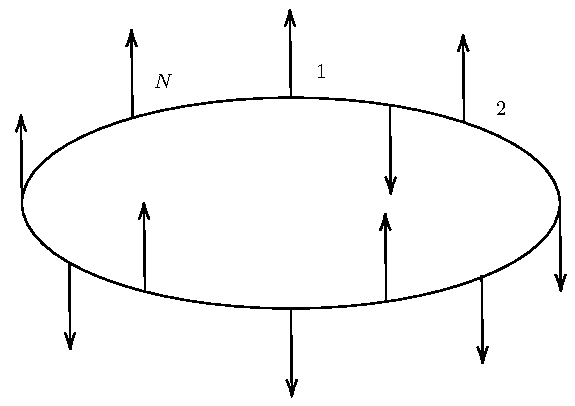
\includegraphics[width=0.5\textwidth]{./img/4__1.pdf}
\caption{\label{fig:6_4} One dimensional lattice ring: Ising model with periodic boundary conditions.}
\end{figure}

Consider the spins sitting on a 1D lattice ring as in Figure \ref{fig:6_4}. The periodic boundary conditions are:
\begin{equation*}
  S_{N+1}=S_1
\end{equation*}
We have:
\begin{equation}
  -\beta \mathcal{H}_ \Omega  ( \{ S \}  ) = K \sum_{i=1}^{N} S_i S_{i+1} + h \sum_{i=1}^{N} S_i
  \label{eq:6_6}
\end{equation}
where
\begin{equation*}
   K \equiv \beta J,  \quad h \equiv \beta H
\end{equation*}
The \( 1-dim \) Ising model with this setup can be solved in several ways. Here we will use the method of the transfer matrix. This is a quite general technique that we will discuss within the Ising model.







%%%%%%%%%%%%%%%%%%%%%%%%%%%%%%%%%%


\subsection{Transfer Matrix method}

Given the Hamiltonian \eqref{eq:6_6}\footnote{The choice of boundary conditions becomes irrelevant in the thermodynamic limit, \( N \rightarrow \infty  \).} we can write the corresponding partition function in the following symmetric form:
\begin{equation*}
  Z_N (k,h) = \sum_{S_1 = \pm 1}^{} \sum_{S_2 = \pm 1}^{}  \dots \sum_{S_N = \pm 1}^{}
  \qty[e^{K S_1 S_2 + \frac{h}{2}(S_1+S_2)} ] \qty[e^{K S_2 S_3 + \frac{h}{2}(S_2+S_3)} ] \dots \qty[e^{K S_N S_1 + \frac{h}{2}(S_N+S_1)} ]
\end{equation*}
We want to write the partition function in a form similarly to \( \sum_{j}^{}  M_{ij} P_{jk} \).
Note that, in the previous form \( Z_N \) can be written as a product of matrices
\begin{equation}
\begin{split}
Z_N (h,k)  &= \sum_{S_1 = \pm 1}^{} \dots \sum_{S_N = \pm 1}^{} \prod_{i=1}^{N} \exp [K S_i S_{i+1} + \frac{h}{2} (S_i + S_{i+1})] \\
& =  \sum_{S_1 = \pm 1}^{} \dots \sum_{S_N = \pm 1}^{} \bra{S_1} \mathbb{T} \ket{S_2} \bra{S_2}  \mathbb{T} \ket{S_3} \dots \bra{S_N}  \mathbb{T} \ket{S_1}
\end{split}
\end{equation}
where \( \mathbb{T} \) is a \( 2 \times 2 \)  matrix defined as
\begin{equation}
  \bra{S} \mathbb{T} \ket{S'} = \exp [K S S' + \frac{h}{2} (S+S')]
\end{equation}
\begin{remark}
  Note that the labels of the matrix corresponds to the values of \( S_i \). Hence, its dimension depends on the number of possible values a spin \( S_i \) can assume.
  It can also depends on how many spins are involved in the interacting terms that are present in the Hamiltonian (\( k_{LL} \sum_{}^{} S_i S_{i+1} S_{i+2} S_{i+3}  \)).
\end{remark}
 For the Ising model, we have \( S_i = \pm 1 \) and nearest neighbour interaction implies that we have two values and that \( \mathbb{T} \) is a \( 2 \times 2 \) matrix whose components are
\begin{subequations}
\begin{align}
  \bra{+1} \mathbb{T} \ket{+1} &= \exp [K+h]  \\
    \bra{+1} \mathbb{T} \ket{-1} &=   \bra{-1} \mathbb{T} \ket{+1} = \exp [-K] \\
      \bra{-1} \mathbb{T} \ket{-1} &=\exp [K-h] 
\end{align}
\end{subequations}
The explicit representation is
\begin{equation}
  \mathbb{T} =
\begin{pmatrix}
e^{K+h}    & e^{-K}  \\
  e^{-K}  & e^{K-h}
\end{pmatrix}
\end{equation}

Let us introduce some useful notations and relations using the bra-ket formalism:
\begin{subequations}
\begin{align}
  \ket{S_i^{(+)}} &= \begin{pmatrix}
  1 \\
  0
  \end{pmatrix}_i
  \quad
  \ket{S_i^{(-)}} = \begin{pmatrix}
  0 \\
  1
  \end{pmatrix}_i   \\
  \bra{S_i^{(+)}} &= (1^*,0)_i \quad   \bra{S_i^{(-)}} = (0,1^*)_i
\end{align}
\end{subequations}
The identity relation is:
\begin{equation}
  \sum_{S_i = \pm 1}^{}  \ket{S_i} \bra{S_i} =
  \ketbra{S_i^{(+)}}{S_i^{(+)}} + \ketbra{S_i^{(-)}}{S_i^{(-)}}
  =\mathbb{1} = \begin{pmatrix}
  1   & 0 \\
  0   & 1
  \end{pmatrix}
\end{equation}
By using the identity property, we can rewrite the partition function as 
\begin{equation}
  \begin{split}
   Z_N (K,h) &= \sum_{S_1 = \pm 1}^{} \dots \sum_{S_N = \pm 1}^{} \bra{S_1} \mathbb{T} \ket{S_2} \bra{S_2}  \mathbb{T} \ket{S_3} \dots \ket{S_i} \bra{S_i}  \mathbb{T} \ket{S_{i+1}} \dots \\
   & = \sum_{S_1 = \pm 1}^{}  \bra{S_1}  \mathbb{T}^N \ket{S_1} = \Tr[\mathbb{T}^N]
     \end{split}
\end{equation}
this is exactly the trace of the matrix, which is most usefully expressed in terms of the eigenvalues. Being \( \mathbb{T} \) symmetric, we can diagonalize it by an unitary transformation as
\begin{equation}
   \mathbb{T}_D = \mathbb{P}^{-1} \mathbb{T} \mathbb{P}
\end{equation}
with \( \mathbb{P} \mathbb{P}^{-1} = \mathbb{1} \). Hence,
\begin{equation*}
\begin{split}
  \Tr[\mathbb{T}^N] &= \Tr[\underbrace{\mathbb{T} \mathbb{T} \mathbb{T} \dots \mathbb{T}}_{N} ] = \Tr[ \mathbb{P} \mathbb{P}^{-1} \mathbb{T} \mathbb{P} \mathbb{P}^{-1} \mathbb{T} \mathbb{P} \dots \mathbb{P}^{-1}  \mathbb{T} \mathbb{P} \mathbb{P}^{-1} ]    \\
  & = \Tr[ \mathbb{P} \mathbb{T}_D^N \mathbb{P}^{-1}] \underset{\substack{ \text{ciclyc property} \\  \text{of the trace} } }{=} \Tr[ \mathbb{T}_D^N \mathbb{P}^{-1} \mathbb{P} ]\\
  & = \Tr[ \mathbb{T}_D^N]
\end{split}
\end{equation*}
where
\begin{equation}
\mathbb{T}_D =  \begin{pmatrix}
  \lambda _+   & 0 \\
  0   & \lambda _-
  \end{pmatrix}
  \quad \Rightarrow \quad
  \mathbb{T}_D^N =  \begin{pmatrix}
    \lambda _+^N   & 0 \\
    0   & \lambda _-^N
    \end{pmatrix}
\end{equation}
with \( \lambda _{\pm} \) are the eigenvalues with \( \lambda _+ > \lambda _- \).
\begin{remark}
\( \mathbb{P} \) is the similitude matrix whose columns are given by the eigenvectors of \(   \lambda _{\pm} \).
\end{remark}
We finally have:
\begin{empheq}[box=\myyellowbox]{equation}
  Z_N (K,h) = \Tr[\mathbb{T_D^N}] = \lambda _+^N  + \lambda _-^N
\end{empheq}
\begin{remark}
As mentioned previously the dimension of the transfer matrix \( \mathbb{T} \) and hence the number of eigenvalues \( \{ \lambda  \}   \) depend both on the possible values of \( S_i \) and on the number of sites involved in terms of the Hamiltonian (range of interaction).
\end{remark}
\begin{example}{}{}
For example, consider the Ising (\( S_i = \pm 1\)) with n. n. and next n. n. interactions. The Hamiltonian is:
\begin{equation*}
  \mathcal{H} = k_1 \sum_{i}^{} S_i S_{i+1} + k_2 \sum_{i}^{} S_i S_{i+1} S_{i+2} S_{i+3}
\end{equation*}
Because of the second term, now there are \( 2^4 = 16 \) possible configurations that can be described by using a \( 4 \times 4 \) transfer matrix that we can write formally as
\begin{equation*}
  \bra{S_i S_{i+1}} \mathbb{T} \ket{S_{i+2} S_{i+3}}
\end{equation*}
\end{example}
\begin{example}{}{}
  For example, suppose \( S_i = +1,0,-1 \), therefore the spin can assume three different values.   This is a \emph{deluted} Ising model.
\end{example}
Now, let us consider the transfer matrix formalism in a more general setting.

\section{General transfer matrix method}
The aim of this section is to describe how transfer matrices can be used to solve classical spin models. The idea is to write down the partition function in terms of a matrix, the transfer matrix. The thermodynamic properties of the model are then wholly described by the eigenspectrum of the matrix. In particular, the free energy per spin in the thermodynamic limit depends only on the largest eigenvalue and the correlation length only on the two largest eigenvalues through simple formulae.

Let \( \mathbb{T} \) be a square matrix \( (n+2) \times (n+2) \) that, for example, it is built if the spin variables may assume \( (n+2) \) possible values. The \emph{k}-esim value can be defined by the bra-ket notation where the two vectors are given by a sequence of "0" and a single "1" at the \emph{k}-esim  position.
\begin{example}{}{}
If \( k=3 \) and there are \( (n+2) \)  possible values:
  \begin{equation*}
    \bra{S_i^{(3)}} = (0,0,1^*,0,\dots,0) \qquad   \ket{S_i^{(3)}} = \begin{pmatrix}
      0 \\
      0 \\
      1 \\
      \vdots \\
      0
      \end{pmatrix}
  \end{equation*}
these are the bra-ket at the \emph{k}-esim position.
\end{example}
Similarly to the \( 2 \times 2 \) Ising case, it is easy to show the identity property
\begin{equation}
  \sum_{S_i}^{} \ket{S_i} \bra{S_i} = \mathbb{1}, \quad \mathbb{1} \in (n+2)\times(n+2)
\end{equation}
where now the sum is over \( (n+2) \) values.

Let us consider  the \emph{diagonal matrix} \( \mathbb{S}_i \), where the elements along the diagonal are all the  \( (n+2) \) possible values of the \emph{i}-esim spin (or of some of their combination if longer interaction terms are considered)
\begin{equation}
  \mathbb{S}_i \equiv  \sum_{S_i}^{} \ket{S_i} S_i \bra{S_i}
\end{equation}
\begin{example}{Ising model \( n+2=2 \)}{}

\begin{equation*}
  \begin{pmatrix}
  1 \\
  0
  \end{pmatrix} S^{(1)} (1^*,0) +
  \begin{pmatrix}
  0 \\
  1
  \end{pmatrix} S^{(2)} (0,1^*) =
  \begin{pmatrix}
  S^{(1)}   & 0 \\
  0   & 0
  \end{pmatrix}
  +
  \begin{pmatrix}
  0   & 0 \\
  0   & S^{(2)}
  \end{pmatrix}
  =
  \begin{pmatrix}
  S^{(1)}  & 0 \\
  0   & S^{(2)}
  \end{pmatrix}
\end{equation*}
Ising: \( S^{(1)} =+1,S^{(2)}=-1 \).






\begin{remark}
Note that in this case the matrix \( \mathbb{S}_i \) is equal to the Pauli matrix \( \sigma _z \).
\end{remark}
\end{example}


\begin{example}{Ising with Vacancies}{}

We have $\sigma_{i} = +1,0,-1$ so we have $n=1$ and $n+2 = 3$.
We can write our vectors as:
$$
\begin{align}
+&1 \to \ket{S_{i}^{(+)}}  &= \begin{pmatrix}
1 \\
0 \\
0
\end{pmatrix}\quad  \bra{S_{i}^{+}} = (1^{*},0,0) \\
&0 \to \ket{S_{i}^{(0)}}  &= \begin{pmatrix}
0 \\
1 \\
0
\end{pmatrix}  \quad \bra{S_{i}^{0}} = (0,1^{*},0)\\
-&1 \to \ket{S_{i}^{(-)}}  &= \begin{pmatrix}
0 \\
0 \\
1
\end{pmatrix} \quad \bra{S_{i}^{-}} = (0,0,1^{*})\\
\end{align}
$$

We then have
$$\mathbb{S}_{i} = \sum_{\sigma_{i} = \pm 1,0} \ket{S_{i}^{(\sigma_{i})}} \sigma_{i}\bra{S_{i}^{(\sigma_{i})}} = \begin{pmatrix}
1 & 0 & 0 \\
0 & 0 & 0 \\
0 & 0 & -1
\end{pmatrix} $$

Show at home that also in this case it is true that
$$\sum \ket{S_{i}^{(\sigma_{i})}} \bra{S_{i}^{(\sigma_{i})}} = \mathbb{1}$$

\end{example}



\begin{remark}
By construction \( \bra{S_i}  \) and \( \ket{S_i}  \) are the eigenvectors related to the eigenvalues \( S_i = S^{(1)},S^{(2)}, \dots,S^{(n+2)} \).
\end{remark}
Similarly. let \( \bra{t_i}  \) and \( \ket{t_i}  \) be the eigenvectors related to the \( (n+2) \) eigenvalues of the transfer matrix \( \mathbb{T} \):
   \( \{ \lambda _+,\lambda _-,\lambda _1,\dots,\lambda _n  \}   \) , with \( \lambda _+ > \lambda _- \ge \lambda _1 \ge \dots \ge \lambda _n \).

Clearly,
\begin{equation}
  \mathbb{T} = \mathbb{P} \mathbb{T}_D \mathbb{P}^{-1} = \sum_{i=1}^{n+2} \ket{t_i} \lambda _i \bra{t_i}
\end{equation}
Indeed
\begin{equation}
  \mathbb{T} \ket{t_j} = \sum_{i=1}^{n+2} \ket{t_i} \lambda _i \braket{t_i}{t_j} = \sum_{i=1}^{n+2}  \ket{t_i} \lambda _i \delta _{ij} = \lambda _j \ket{t_j}
\end{equation}
Given the set of \( \lambda  \) described above, the \emph{N} particle partition function is given by
\begin{empheq}[box=\myyellowbox]{equation}
  Z_N  = \lambda _+^N +\lambda _-^N + \sum_{i=1}^{n} \lambda _i^{N}
  \label{eq:7_01}
\end{empheq}

\subsection{The free energy}


Now, let us consider the free energy 
\begin{equation*}
  F_N = -k_B T \log{Z_N} 
\end{equation*}
In particular, we are interested in the limit of the bulk free energy. Looking at the thermodynamic limit \( N \rightarrow \infty  \) we have
\begin{equation*}
  f_b  = \lim_{N \rightarrow \infty } \frac{1}{N} F_N = \lim_{N \rightarrow \infty } \frac{1}{N} (-k_B T) \log{\qty[\lambda _+^N + \lambda _-^N + \sum_{i=1}^{n} \lambda _i ^N  ] }
\end{equation*}
by factorizing \( \lambda _+ \), we obtain
\begin{equation*}
  f_b = \lim_{N \rightarrow \infty } \frac{-k_B T}{N} \log{\qty[\lambda _+^N \qty(1+\frac{\lambda _-^N}{\lambda _+^N}+ \sum_{i=1}^{n} \qty(\frac{\lambda _i}{\lambda _+})^N    ) ] }
\end{equation*}
Since \( \lambda _+ > \lambda _- > \lambda _1 > \dots \lambda _n \),
\begin{equation*}
\qty(\frac{\lambda _-}{\lambda _+})^N \overset{N \rightarrow \infty }{\longrightarrow} 0,
\quad
\qty(\frac{\lambda _i}{\lambda _+})^N \overset{N \rightarrow \infty }{\longrightarrow} 0
\quad \forall i
\end{equation*}
The result is 
\begin{empheq}[box=\myyellowbox]{equation}
f_b = -k_B T \log{\lambda _+}
\end{empheq}
The \emph{limiting bulk free-energy depends only on the largest eigenvalue of the transfer matrix \( \mathbb{T} \)}! This is important since sometimes it is much simpler to compute only the largest eigenvalue than the whole spectrum of \( \mathbb{T} \). Also an important theorem about \( \lambda _+ \) exists.

  \begin{theorem}{Perron-Frobenius}{}
  Let \( \mathbb{A} \) be a \( n \times n \) matrix. If \( \mathbb{A} \) is finite (\( n < \infty  \)) and \( \mathbb{A}_{ij} > 0 , \forall i,j \), \( (\mathbb{A}_{ij}=\mathbb{A}_{ij} (\va{x})) \), therefore its largest eigenvalue \( \lambda _+ \) has the following properties:
  \begin{enumerate}
  \item \( \lambda _+ \in \R^+  \)
  \item \( \lambda _+ \neq \text{ from } \{ \lambda _i \}_{i=1,\dots, n-1 }   \). It means there is no degeneracy.
  \item \( \lambda _+ \) is a analytic function of the parameters of \( \mathbb{A} \).
  \end{enumerate}
  \end{theorem}

\begin{remark}
Since in our case \( \mathbb{A} \leftrightarrow  \mathbb{T} \), \( \lambda _+ \) is related to \( f_b \) from the theorem. This means that \( f_b \) is an analytic function!
\end{remark}
If the conditions of the Perron-Frobenius theorem are satisfied by \( \mathbb{T} \), the model described by  \( \mathbb{T} \) cannot display a phase transition!
\begin{remark}
This is true for \( T>0 \) since for \( T=0 \) some \( \mathbb{T}_{ij} \) can be either 0 or \( \infty  \) violating the hypothesis of the theorem.
\end{remark}
\begin{remark}
If \( \mathbb{T} \) has infinite dimension (see \( d>1 \)) the hypothesis of the theorem are not valid anymore and \( f_b \) can be non-analytic.
\end{remark}


\subsection{The correlation function}
A second important quantity which is simply related to the eigenvalues of the transfer matrix is the correlation length. To calculate this, we need the spin-spin correlation function which serves as an example of how to obtain averages of products of spins using transfer matrices.

Let us consider the two point correlation between two spins at distance \emph{R} to another. The fluctuation with respect to the average is:
\begin{empheq}[box=\myyellowbox]{equation}
  \Gamma _R \equiv  \expval{S_1 S_R} - \expval{S_1}\expval{S_R}
\end{empheq}
Since
\begin{equation*}
  \Gamma _R \underset{R \rightarrow \infty }{\sim } \exp [-R/\xi ]
\end{equation*}
we can define the correlation length \( \xi  \) as
\begin{empheq}[box=\myyellowbox]{equation}
  \xi^{-1} \equiv  \lim_{R \rightarrow \infty } \qty[ - \frac{1}{R} \log{ \qty| \expval{S_1 S_R} - \expval{S_1}\expval{S_R}| } ]
  \label{eq:7_2}
\end{empheq}
Now, let us compute the terms \( \expval{S_1 S_R}_N  \) and \( \expval{S_1}_N\expval{S_R}_N \).

\subsubsection{Term \(\expval{S_1 S_R}_N\)}
\noindent From the definition of average we obtain
\begin{equation}
  \expval{S_1 S_R}_N = \frac{1}{Z_N} \sum_{\{ S \}  }^{} S_1 S_R \exp [-\beta \mathcal{H}_N]
\end{equation}
\begin{remark}
The subscript \( N \) denotes that we are again considering a ring of \( N \) spins. \( Z_N \) is known from equation \eqref{eq:7_01}.
\end{remark}
Writing this expression by using the transfer matrix formalism, one obtains
\begin{equation*}
\expval{S_1 S_R}_N  = \frac{1}{Z_N} \sum_{\{ S \}  }^{} S_1 \bra{S_1} \mathbb{T} \ket{S_2} \dots  \bra{S_{R-1}} \mathbb{T} \ket{S_R} S_R \bra{S_R} \mathbb{T} \ket{S_{R+1}} \dots \bra{S_N} \mathbb{T} \ket{S_1}
\end{equation*}
Summing over the free spins,
\begin{equation}
  \expval{S_1 S_R}_N = \frac{1}{Z_N} \sum_{S_1,S_R}^{} S_1 \bra{S_1} \mathbb{T}^{R-1} \ket{S_R} S_R \bra{S_R} \mathbb{T}^{N-R+1} \ket{S_1}
  \label{eq:7_1}
\end{equation}
On the other hand, since
\begin{equation*}
  \mathbb{T} = \sum_{i=1}^{n+2} \ket{t_i} \lambda _i  \bra{t_i}
\end{equation*}
we have
\begin{subequations}
\begin{align}
  \mathbb{T}^{R-1} &= \sum_{i=1}^{n+2} \ket{t_i} \lambda _i^{R-1}  \bra{t_i} \\
    \mathbb{T}^{N-R+1} &= \sum_{i=1}^{n+2} \ket{t_i} \lambda _i^{N-R+1}  \bra{t_i}
\end{align}
\end{subequations}
Hence,
\begin{subequations}
\begin{align}
  \bra{S_1} \mathbb{T}^{R-1} \ket{S_R} & = \sum_{i=1}^{n+2} \braket{S_1}{t_i} \lambda_i ^{R-1} \braket{t_i}{S_R} \\
  \bra{S_R} \mathbb{T}^{N-R+1} \ket{S_1} & = \sum_{j=1}^{n+2} \braket{S_R}{t_j} \lambda_j ^{N-R+1} \braket{t_j}{S_1}   
\end{align}
\end{subequations}
and plugging these expressions in  \eqref{eq:7_1} one gets
\begin{equation*}
  \sum_{\{ S \}  }^{}  S_1 S_R e^{-\beta \mathcal{H}_N} = \sum_{S_1 S_R}^{} S_1 \sum_{i=1}^{n+2} \braket{S_1}{t_i} \lambda _i^{R-1} \braket{t_i}{S_R} S_R \sum_{j=1}^{n+2} \braket{S_R}{t_j} \lambda_j ^{N-R+1} \braket{t_j}{S_1}
\end{equation*}
Since the term \( \braket{t_j}{S_1}  \) is a scalar, it can be moved at the beginning of the product. Remembering the notations
\begin{subequations}
\begin{align}
  \mathbb{S}_1 &= \sum_{S_1}^{} \ket{S_1} S_1 \bra{S_1} \\
  \mathbb{S}_R &= \sum_{S_R}^{} \ket{S_R} S_R \bra{S_R}
\end{align}
\end{subequations}
one gets
\begin{equation}
  \sum_{\{ S \}  }^{}  S_1 S_R e^{-\beta \mathcal{H}_N}= \sum_{ij}^{} \bra{t_j } \mathbb{S}_1 \ket{t_i} \lambda _i^{R-1} \bra{t_i} \mathbb{S}_R \ket{t_j} \lambda _j ^{N-R+1}
\end{equation}


%%%%%%%%%%%%%%%%%%%%%%%%%%%%%%%%%%%%%%%%%%%%%%%%%%%%%%%%%%%%%%%%%%%%%%%%%%%%%%%%%%%%%%%%%%%%%%%


\noindent Since \( \sum_{k}^{} \lambda _k^N = Z_N \) for \( k=+,-,1,\dots,n \), we have
\begin{equation*}
  \expval{S_1 S_R}_N = \frac{\sum_{ij}^{} \bra{t_j} \mathbb{S}_1 \ket{t_i} \lambda _i^{R-1} \bra{t_i} \mathbb{S}_R \ket{t_j} \lambda _j^{N-R+1}      }{\sum_{k=1}^{n} \lambda _k^N  }
\end{equation*}
If we now multiply and divide by \( \lambda _+^N \), we get
\begin{equation*}
  \expval{S_1 S_R}_N = \frac{\sum_{ij}^{} \bra{t_j} \mathbb{S}_1 \ket{t_i} (\lambda _i/ \lambda _+)^{R-1}  \bra{t_i} \mathbb{S}_R \ket{t_j} (\lambda _j / \lambda _+)^{N-R+1}    }{\sum_{k=1}^{n} (\lambda _k  / \lambda _+)^{N} }
\end{equation*}
\begin{remark}
In the thermodynamic limit \( N \rightarrow \infty  \), only the terms with \( j=+ \) and \( k=+ \) will survive in the sum. Remind that \( R \) is fixed.
\end{remark}
\begin{equation*}
\expval{S_1 S_R} =   \lim_{N \rightarrow \infty } \expval{S_1 S_R}_N = \sum_{i= \pm,1 \dots n}^{} \qty(\frac{\lambda _i}{\lambda _+})^{R-1} \bra{t_+} \mathbb{S}_1 \ket{t_i} \bra{t_i} \mathbb{S}_R \ket{t_+}
\end{equation*}
Rembember that \( \lambda _+ > \lambda _- \ge \lambda _1 \ge \dots \ge \lambda _n \):
\begin{equation*}
  \expval{S_1 S_R} = \bra{t_+} \mathbb{S}_1 \ket{t_+} \bra{t_+} \mathbb{S}_R \ket{t_+} +   \sum_{i \neq +}^{n} \qty(\frac{\lambda _i}{\lambda _+})^{R-1} \bra{t_+} \mathbb{S}_1 \ket{t_i} \bra{t_i} \mathbb{S}_R \ket{t_+}
\end{equation*}
Since one can prove 
\begin{equation}
  \lim_{N \rightarrow \infty } \expval{S_R}_1 = \bra{t_+} \mathbb{S}_1 \ket{t_+} , \quad \lim_{N \rightarrow \infty } \expval{S_R}_N = \bra{t_+} \mathbb{S}_R \ket{t_+}
  \label{eq:8_3}
\end{equation}
we obtain
\begin{equation}
  \expval{S_1 S_R} = \expval{S_1} \expval{S_R} + \sum_{i \neq +}^{}  \qty(\frac{\lambda _i}{\lambda _+})^{R-1} \bra{t_+} \mathbb{S}_1 \ket{t_i} \bra{t_i} \mathbb{S}_R \ket{t_+}
  \label{eq:8_2}
\end{equation}
\begin{example}{Show relation \eqref{eq:8_3}}{}
Let us prove \eqref{eq:8_3} by a method analogous to that followed above.
\begin{equation*}
\begin{split}
\expval{S_1}_N &= \frac{1}{Z} \sum_{\{ S \} }  S_1 e^{- \beta \mathcal{H}_N}
= \frac{1}{Z} \sum_{S_1} S_1 \bra{S_1}  \mathbb{T}^N \ket{S_1} 
 = \frac{1}{Z} \sum_{S_1} S_1 \sum_{i}  \bra{S_1}\ket{t_i} \lambda_i^N \bra{t_i} \ket{S_1} \\
&= \frac{1}{Z} \sum_{i} \lambda_i^N \bra{t_i} \mathbb{S}_1 \ket{t_i}  
 = \frac{\sum_{i}^{} \qty(\lambda_i/\lambda_+)^N \bra{t_i} \mathbb{S}_1 \ket{t_i}  }{ \sum_{k=1}^{n} (\lambda _k  / \lambda _+)^{N} }
\end{split}
\end{equation*}
Taking the limit \( N \rightarrow \infty \):
\begin{equation*}
\expval{S_1} =   \lim_{N \rightarrow \infty } \expval{S_1}_N = 
\bra{t_+} \mathbb{S}_1 \ket{t_+}
\end{equation*}
\end{example}
The correlation function follows immediately from \eqref{eq:8_2},
\begin{equation}
\Gamma _R =   \expval{S_1 S_R} - \expval{S_1}\expval{S_R} = \sum_{i \neq +}^{n} \qty(\frac{\lambda _i}{\lambda _+})^{R-1} \bra{t_+} \mathbb{S}_1 \ket{t_i} \bra{t_i} \mathbb{S}_R \ket{t_+}
\end{equation}
\begin{remark}
\( \Gamma_R \) depends only on the eigenvalues and eigenvectors of the transfer matrix \( \mathbb{T} \) and by the values of the spins \( S_1 \) and \( S_R \).
\end{remark}
A much simpler formula is obtained for the correlation length \eqref{eq:7_2}. Taking the limit \( R \rightarrow \infty  \) the ratio \( (\lambda _-/ \lambda _+) \) dominates the sum and hence
\begin{equation*}
\begin{split}
\xi ^{-1} &=  \lim_{R \rightarrow \infty } \qty{-\frac{1}{R-1} \log{\qty|\expval{S_1S_R} - \expval{S_1} \expval{S_R}   |} } \\
& = \lim_{R \rightarrow \infty }  \qty{-\frac{1}{R-1} \log{\qty[  \qty(\frac{\lambda _-}{\lambda _+})^{R-1} \bra{t_+} \mathbb{S}_1 \ketbra{t_-}{t_-} \mathbb{S}_R \ket{t_+}  ]  } } \\
& = -\log{\qty[\qty(\frac{\lambda _-}{\lambda _+}) ] } - \lim_{R \rightarrow \infty } \frac{1}{R-1} \log{ \bra{t_+} \mathbb{S}_1 \ketbra{t_-}{t_-} \mathbb{S}_R \ket{t_+}    }  \\
& = - \log{\qty(\frac{\lambda _-}{\lambda _+}) }
\end{split}
\end{equation*}
The important result is
\begin{empheq}[box=\myyellowbox]{equation}
  \xi ^{-1} = -  \log{\qty(\frac{\lambda _-}{\lambda _+}) }
\end{empheq}
It means that the \emph{correlation length does depend only on the ratio between the two largest eigenvalues of the transfer matrix \( \mathbb{T} \)}.


\subsection{Results for the \emph{1-dim} Ising model}
Let us now return to the example of the nearest neighbour Ising model in a magnetic field, to obtain explicit results for the bulk free energy \(f_b\), the correlation function \( \Gamma\) and the correlation length \( \xi \).

Recall that the transfer matrix of such a system is given by
\begin{equation*}
  \mathbb{T} =
  \begin{pmatrix}
  \exp (K+h)     & \exp (-K)  \\
  \exp (-K)    & \exp (K-h)
  \end{pmatrix}
\end{equation*}
Now, let us calculate the eigenvalues:
\begin{equation*}
  \abs{\mathbb{T}-\lambda \mathbb{1}} =  (e^{K+h}- \lambda  )(e^{K-h}-\lambda  )-e^{-2K}=0
\end{equation*}
The two solutions are
\begin{empheq}[box=\myyellowbox]{equation}
  \lambda _{\pm} = e^{K} \cosh(h) \pm \sqrt{e^{2K}\sinh^2 (h)+e^{-2K} }
\end{empheq}
\subsubsection{The free energy}
The free energy is
\begin{equation*}
\begin{split}
    f_b & \equiv \lim_{N \rightarrow \infty } \frac{-k_B T}{N} \log{Z_N (K,h)}   \\
    & = -k_B T \lim_{N \rightarrow \infty } \frac{1}{N}  \log{\qty[\lambda _+^N \qty(1+\qty(\frac{\lambda _-}{\lambda _+})^N ) ] } \\
    & = -k_B T \log{\lambda _+}
\end{split}
\end{equation*}
and inserting the explicit expression of \( \lambda _+ \) for the Ising model, we get
\begin{equation}
\begin{split}
f_b  &=  -k_B T \log{ \qty( e^{K} \cosh h + \sqrt{e^{2K} \sinh^2 (h) + e^{-2K}  } ) } \\
& = -K k_B T - k_B T \log{\qty( \cosh(h)+\sqrt{\sinh^2(h)+e^{-4K}  } )}
\end{split}
\end{equation}
\begin{remark}
Remember that \( K \equiv \beta J, h \equiv \beta H\).
\end{remark}
\begin{exercise}{}{}
Check that if \( h=0 \) we get back the expression found previously with the iterative method. What is the importance of boundary conditions?
\begin{solution}
If \(h=0\), we obtain 
\begin{equation*}
\begin{split}
   f_b &= - K k_B T - k_B T \log ( 1 + \frac{1}{e^{2K}})
   = -k_B T \qty( \log e^K  +  \log ( 1 +  e^{-2K}) ) \\ 
   & = -k_B T  \log ( e^K  +  e^{-K} ) =   -k_B T  \log (2 \frac{ e^K  +  e^{-K} }{2} ) \\
   & =  -k_B T  \log (2 \cosh K ) = -k_B T  \log ( 2 \cosh (\frac{J}{k_B T }) )
\end{split}   
\end{equation*}
The choice of boundary conditions becomes irrelevant in the thermodynamic limit, \(N \rightarrow \infty\).
\end{solution}
\end{exercise}
Let us now consider the limits \( T \rightarrow 0 \) and \( T \rightarrow \infty  \) by keeping \emph{H} fixed and \emph{J} fixed.
\begin{itemize}
\item Case: \( T \rightarrow 0  \Rightarrow K \rightarrow \infty , h \rightarrow \infty  \).
\begin{subequations}
\begin{align*}
  e^{-4K} & \overset{K \rightarrow \infty }{\longrightarrow} 0  \\
  \sqrt{\sinh^2 h} & \overset{h \rightarrow \infty }{\sim } \sinh (h)
\end{align*}
\end{subequations}
We have 
\begin{equation*}
\cosh h + \sinh h \sim \frac{2 e^{h} }{2} \simeq e^{h}
\end{equation*}
and
\begin{equation}
  f \overset{\substack{h \rightarrow \infty  \\ K \rightarrow \infty  } }{\sim } - K k_B T - k_B T \log{e^{h} } \sim -J -H \quad const
\end{equation}
Therefore, as \( T \rightarrow 0^+ \), \emph{f} goes to a constant that depends on \emph{J} and \emph{H}.

\item  Case: \( T \rightarrow \infty   \Rightarrow K \rightarrow 0 , h \rightarrow 0  \).
In this case we suppose also that \emph{H} and \emph{J} (fixed) are also finite.
\begin{subequations}
\begin{align*}
  e^{-4K} & \simeq 1  \\
  \sqrt{\sinh^2 h + e^{-4K} } & \sim \sqrt{1}
\end{align*}
\end{subequations}
Since \( \cosh h \overset{h \rightarrow 0}{\sim } 1  \):
\begin{equation}
  f_B \sim  -K k_B T - k_B T \log{(1+1)} \sim  -J -k_B T \ln{2}
\end{equation}
Therefore, as \( T \rightarrow \infty  \), the free energy goes linearly to zero, as in Figure \ref{fig:8_1}.

\textbf{WHYYYYYYYYYY}


\begin{figure}[h!]
\centering
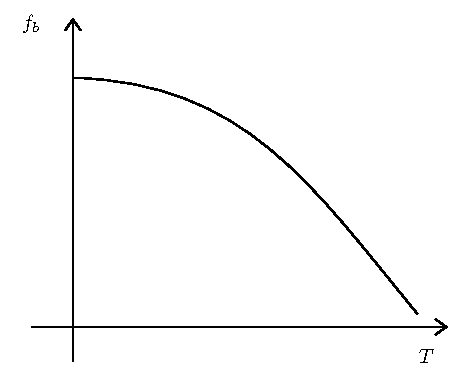
\includegraphics[width=0.5\textwidth]{./img/1.pdf}
\caption{\label{fig:8_1} Plot of the free energy \( f_b \) in function of the temperature \( T \). For \( T \rightarrow 0 \), the free energy becomes constant, while for \( T \rightarrow \infty  \) it goes linearly to zero.  }
\end{figure}
\end{itemize}

\subsubsection{The magnetization}
This can be obtained by differentiating the negative of the free energy with respect to the magnetic field \( H \) (or by using equation \eqref{eq:8_3}):
\begin{equation*}
  m = - \pdv{f_b}{H} = - \frac{1}{k_B T } \pdv{f_b}{h} = \pdv{}{h} \qty[  \log{\qty( \cosh(h)+\sqrt{\sinh^2(h)+e^{-4K}  } )} ]
\end{equation*}
The result is
\begin{equation}
  m =   \frac{\sinh h + \frac{ \sinh h \cosh h}{\sqrt{\sinh^2 h + e^{-4K} }} }{\cosh h + \sqrt{\sinh^2 h + e^{-4K} } } 
  = \frac{\sinh h  }{\sqrt{\sinh^2 h + e^{-4K} } }
  \label{eq:8_1}
\end{equation}
\begin{itemize}
\item Case: \( T>0 \) fixed, \( H \rightarrow 0 \Rightarrow h \rightarrow 0\).
\begin{subequations}
\begin{align*}
  \sinh h & \sim h \sim 0, \\ \cosh h &\sim 1
\end{align*}
\end{subequations}
In zero field \( h \rightarrow 0 \), we have \( m \rightarrow 0 \) for all \( T>0 \). It means that there is no spontaneous magnetization!
\end{itemize}


\subsubsection{The magnetic susceptibility}
\begin{equation}
  \chi_T  \equiv  \pdv{m}{H} = \frac{1}{k_B T} \pdv{m}{h}
\end{equation}
If we consider the case \( h \ll 1 \), it is convenient first expand the  \eqref{eq:8_1} for \( h \rightarrow 0 \) and take the derivative to get \( \chi _T \).

Since \( \sinh (h) \sim h+h^3 \) and \( \cosh (h) \sim 1 + h^2 \), we have
\begin{equation*}
  m \overset{h \ll 1}{\sim } \frac{h (1+e^{2K} )}{1+e^{-2K} }
\end{equation*}
If we now derive with respect to \emph{h}

\begin{equation*}
\chi_{T} = \frac{\cosh(h)}{\sqrt{ \sinh^{2}(h) + e^{-4K} } (1 + e^{4K}\sinh^{2}(h))}
\end{equation}
In the case of $h\ll1$:
\begin{equation*}
 \chi _T = \frac{1}{k_B T} \pdv{m}{h} \overset{h \ll 1}{\approx } \frac{1}{k_B T} \frac{(1+e^{2K} )}{(1+e^{-2K} )}
\end{equation*}
\begin{itemize}
\item Case: \( T \rightarrow \infty  \Rightarrow K \rightarrow 0\).
\begin{equation*}
  e^{2K} \simeq e^{-2K} \simeq 1
\end{equation*}
The \textit{Curie's Law} for paramagnetic systems is:
\begin{empheq}[box=\myyellowbox]{equation}
  \chi _T \sim \frac{1}{k_B T}
\end{empheq}
\item Case: \( T \rightarrow 0 \Rightarrow K \rightarrow \infty  \).
\begin{equation*}
  e^{-2K} \simeq 0
\end{equation*}

\begin{empheq}[box=\myyellowbox]{equation}
  \chi _T \sim \frac{1}{k_B T} e^{2K} \sim  \frac{1}{k_B T} e^{2J/k_B T}
\end{empheq}
\end{itemize}

\subsubsection{The correlation length}
\begin{equation}
  \xi ^{-1} = -\log{\qty(\frac{\lambda _-}{\lambda _+}) } = - \log{\qty[ \frac{\cosh h - \sqrt{\sinh^2 h + e^{-4K} } }{\cosh h + \sqrt{\sinh^2 h + e^{-4K} }}] }
\end{equation}
For \( h=0 \), we have \( \cosh h \rightarrow 1, \sinh h \rightarrow 0 \):
\begin{equation*}
  \xi ^{-1} = - \log{\qty[\frac{1- e^{-2K} }{1+ e^{-2K} }] } =  - \log{\qty[\frac{1 }{\coth K }] }
\end{equation*}
Therefore:
\begin{equation}
  \xi = \frac{1}{\log{ (\coth K )} }, = -\frac{1}{\log{ (\tanh K )} }, \quad \text{for } h = 0
\end{equation}
\begin{itemize}
\item Case: \( T \rightarrow 0 \Rightarrow K \rightarrow \infty  \).
\begin{equation*}
  \coth K = \frac{e^{K} + e^{-K}  }{e^{K} - e^{-K}  } \overset{K \rightarrow \infty }{\simeq} 1 + 2 e^{-2K} + \dots \quad \overset{K \rightarrow \infty }{ \longrightarrow  } 1
\end{equation*}
It implies
\begin{equation*}
  \xi \overset{K \gg 1}{\sim } \frac{1}{\ln{(1+ 2 e^{-2K} )} } \sim \frac{e^{2K} }{2}
\end{equation*}
Hence,
\begin{equation}
  \xi \overset{T \rightarrow 0}{\sim } \frac{1}{2} e^{J/k_B T}
\end{equation}
It diverges exponentially \( \xi  \rightarrow \infty  \) as \( T \rightarrow 0 \).
\item Case: \( T \rightarrow \infty \Rightarrow K \rightarrow 0 \).
\begin{equation*}
  \coth K = \frac{e^{K} + e^{-K}  }{e^{K} - e^{-K}  } \overset{K \rightarrow 0 }{\simeq}
  \frac{1+K+\frac{K^2}{2}+1-K+\frac{K^2}{2}}{1+K+\frac{K^2}{2}-1+K-\frac{K^2}{2}}
  \sim \frac{2+2 \frac{K^2}{2}}{2K} \sim \frac{1+K^2}{K}
\end{equation*}
\begin{equation*}
  \xi ^{-1} = \log{(\coth K)} \overset{K \rightarrow 0}{\sim } \ln{\frac{1}{K}} + \ln{(1+K^2)} \sim + \infty
\end{equation*}
Therefore
\begin{equation*}
  \xi  \overset{K \rightarrow 0}{\longrightarrow} 0
\end{equation*}
More precisely,
\begin{equation}
  \xi \overset{K \rightarrow 0}{\sim } \frac{1}{\ln{(1/K)} + \ln{(1+K^2)}  } \overset{K \rightarrow 0}{\sim } - \frac{1}{\ln{K} }
\end{equation}

\end{itemize}


\section{Fluctuation-response for Ising-like models}

We have an Hamiltonian like:
$$\mathcal{H}_{N} = -J \sum_{\avg{{ij}} }s_{i}s_{j} - \sum_{i}H_{i}s_{i}$$
And a partition function like this:
$$Z_{N} = \underset{\{ s \}}{\text{Tr}}\exp(-\beta \mathcal{H}_{N})$$
If we compute the magnetisation we get:
$$M_{i} = \avg{s_{i}} _{N} = \frac{1}{\beta Z_{N}} \frac{ \partial Z_{N} }{ \partial H_{i} } = \frac{1}{\beta} \frac{ \partial  \ln Z_{N} }{ \partial H_{i} } $$
So if we write the correlation function in this case is:
$$\avg{s_{i}s_{j}}_{N} = \frac{1}{\beta^{2}} \frac{1}{Z_{N}} \frac{ \partial^{2} Z_{N} }{ \partial H_{i}\partial H_{j} } $$
The connected correlation function then is:
$$
G_{c}(i,j) = \avg{s_{i}s_{j}}_{c} = \avg{s_{i}s_{j}}  - \avg{s_{i}} \avg{s_{j}} = \frac{1}{\beta^{2}}\frac{ \partial^{2}\ln Z_{N} }{ \partial H_{i}\partial H_{j} }
$$
\begin{remark}
In general, differentiating $Z_{N}$ to order $k$ gives the $k$-point correlation function. So our partition function is the generating function of the correlations and the free-energy is the generating function of the connected correlations.
\end{remark}
Setting $H_{i} = 0$ AFTER having taken the derivative gives:
$$
G_{c}(i,j)\bigg\rvert_{H_{i}=0} = \avg{s_{i}s_{j}} - \avg{s_{i}} \avg{s_{j}} = \frac{1}{\beta^{2}}\frac{ \partial^{2}\ln Z_{n} }{ \partial H_{i}\partial H_{j} }\bigg\rvert_{H_{i}= 0} 
$$
That gives:
$$\frac{ \partial M_{i} }{ \partial H_{j} } = \frac{1}{\beta}\frac{ \partial ^{2}\ln Z_{N} }{ \partial H_{i}H_{j} } = \beta G_{c}(i,j) $$
This is the first form of the \textbf{Fluctuation-Response Relation}.
\subsection*{Spin Susceptibility}
$\chi_{N}$ in a uniform magnetic field $H_{i} = H_{i}(H) = H$ 
$$\frac{ \partial M_{i} }{ \partial H }  = \sum_{j} \frac{ \partial M_{i} }{ \partial H_{j} } \frac{ \partial H_{j} }{ \partial H } = \beta \sum_{j}G_{c}(i,j)$$
So
$$\chi = \frac{ \partial M }{ \partial H } = \beta \sum_{j}G_{c}(i,j) = \frac{\beta}{N}\sum_{i,j} G_{c}(i,j)$$
\begin{remark}
$M = \avg{s_{i}}$ is independent on $i$ (it's translation invariant) so it is $\sum_{j}G_{c}(i,j)$ independent of $i$
\end{remark}






\section{Classical Heisenberg model for \emph{d=1} }

The Quantum Heisenberg Model is defined by the Hamiltonian Operator:
$$\mathcal{H} = - J \sum_{\avg{ij} } \vec{s_{i}}\cdot \vec{S_{j}} = - J \sum_{ij} (S_{i}^{x}S_{j}^{x} + S_{i}^{y}S_{j}^{y} + S_{i}^{z}S_{j}^{z})$$

Since the different component $S_{x},S_{y},S_{z}$ do not commute the full problem is not solvable analytically.
On the other hand one can look at the associated model in which $\mid \vec{S}\mid$ goes to infinity and in the simples case of $d = 1$.



\subsection{Classical Heisenberg Chain}
Let us consider the Hamiltonian
$$\mathcal{H} = - J \sum_{i=1}^{N} \vec{S_{i}} \cdot \vec{S}_{i+1}$$
where the spins have infinite magnitude i.e. $\mid \vec{S}\mid \to \infty$.
We introduce the unit vector operator:
$$s_{i} = \frac{\vec{S}_{i}}{\mid \vec{S}\mid}$$
It's commutation rules are:
$$\begin{align}
[s^{x}_{i},s_{i}^{y}] = i \frac{s_{i}^{z}}{S} \\
[s^{y}_{i},s_{i}^{z}] = i \frac{s_{i}^{x}}{S} \\
[s^{z}_{i},s_{i}^{x}] = i \frac{s_{i}^{y}}{S}
\end{align}$$
Where $S = \mid \vec{S}\mid$.
In the limit $S \to \infty$ the components commute and the hamiltonian form can be written in classical form:
$$\mathcal{H} = - J\sum_{i}^{N} \vec{s}_{i} \cdot \vec{s}_{i+1}$$
Where $J = J_{s}S^{2}$.
Note that now the spins are unit length vectors, so they are continuous values on the unit sphere.
Let us consider periodic boundary conditions $s_{N+1} = s_{1}$ and $h = 0$. We can rewrite the Hamiltonian as:
$$-\beta \mathcal{H}(\{ \vec{s} \}) = K \sum_{i=1}^{N}\vec{s}_{i}\cdot \vec{s}_{i+1}$$
The model satisfies $O(3)$ symmetry. We can then write the partition function:
$$Z_{N} = \sum_{\{ \vec{s} \}} \exp[-\beta \mathcal{H}(\{ \vec{s} \})] = \int \frac{d\Omega_{1}}{4\pi}\int \frac{d\Omega_{2}}{4\pi}\dots\int \frac{d\Omega_{N}}{4\pi}\prod_{i=1}^{N} \exp(K \vec{s}_{i}\cdot \vec{s}_{i+1})$$
where the $d\Omega_i$ is the element of the solid angle for the unit vector $\vec{s}_{i}$.
To compute $Z_{N}$ one can either compute the integrals above (in spherical coordinates) or by using the Transfer Matrix Formalism

\subsubsection*{Transfer Matrix Formalism}






In the transfer matrix formalism\footnote{Here we use $\va{S}$ but is the same as before}:

\begin{equation}
  Z_N (K) = \sum_{\{ \va{S} \}  }^{} e^{-\beta \mathcal{H}} = \sum_{\{ \va{S} \}  }^{} e^{K \sum_{i=1}^{N} \va{S}_i \vdot \va{S}_{i+1} } = \Tr(\mathbb{T}^N)
\end{equation}
where 
\begin{equation*}
\bra{\va{S}_i} \mathbb{T} \ket{\va{S}_{i+1}} = e^{K \va{S}_i \vdot \va{S}_{i+1}} 
\end{equation*}
Similarly to the Ising case, 
\begin{equation*}
  \mathbb{T} = \sum_{i}^{} \ket{t_i} \lambda _i \bra{t_i}
\end{equation*}
and
\begin{equation*}
  \mathbb{T}_D = \mathbb{P}^{-1} \mathbb{T}\mathbb{P}
\end{equation*}
The problem is computing the eigenvalues \( \lambda _i \) of \( \mathbb{T} \).

Formally, we should find
\begin{equation*}
  \exp [K \va{S}_1\vdot \va{S}_{2}] = \bra{\va{S}_1} \mathbb{T} \ket{\va{S}_2} = \sum_{i \in \text{\tiny eigenvalues}}^{} \lambda _i \braket{\va{S}_1}{t_i}  \braket{t_i}{\va{S}_2}
  = \sum_{i}^{} \lambda _i f_i ( \va{S}_1) f^* (\va{S}_2)
\end{equation*}

\begin{remark}
  We start by noticing that the term \( e^{K \va{S}_1 \cdot \va{S}_2}  \) is similar to the plane wave \(e^{i \va{q}\vdot \va{r}}  \), that in scattering problems is usually expanded in spherical coordinates. Plane wave can be expanded as a sum of spherical harmonics as
  \begin{equation*}
    e^{i \va{q}\vdot \va{r}} = 4 \pi \sum_{l=0}^{\infty } \sum_{m=-l}^{l} (i)^l j_l (qr) Y_{lm}^* (\vu{q}) Y_{lm} (\vu{r})
  \end{equation*}
  where
  \begin{equation*}
    j_l (qr) = - \frac{(i)^l}{2} \int_{0}^{\pi} \sin(\theta ) e^{i q r \cos(\theta ) } P_l (\cos(\theta ) ) \dd[]{\theta }
  \end{equation*}
  are the \emph{spherical Bessel functions}, while  the \( P_l (\cos(\theta ) ) \) are the \emph{Legendre polynomial} of order \emph{l}.
\end{remark}

From a formal comparison we have
  \begin{equation}
    \va{S}_1 \leftrightarrow \vu{S}_1, \qquad
      \begin{cases}
           i \va{q}\cdot \va{r} = iqr \\
           K \va{S}_1 \cdot \va{S}_2 = K \abs{\va{S}_1} \abs{\va{S}_2} = K
      \end{cases}
  \end{equation}
  multiplying by \( (-i) \)  we can write
  \begin{equation}
    qr = -iK \abs{\va{S}_1} \abs{\va{S}_2} = -iK
  \end{equation}
  In our case, we have
  \( \vu{q} = \va{S}_1, \vu{r} = \va{S}_2 \). Hence,
  \begin{equation}
    e^{K \va{S}_1 \cdot \va{S}_2} = 4 \pi  \sum_{l=0}^{\infty } \sum_{m=-l}^{l} (i)^l j_l (-iK) Y_{lm}^* (\va{S}_1) Y_{lm} (\va{S}_2) = \sum_{i}^{} \lambda _i f_i (\va{S}_1) f^* (\va{S}_2)
  \end{equation}
where
\begin{equation}
  \lambda _i = \lambda _{lm} (K) = 4 \pi (i)^l j_l (-iK)
\end{equation}
\begin{remark}
Note that \( \lambda _i \) does not depend on \emph{m}!
\end{remark}


If \( l=0 \), the largest eigenvalue is:
\begin{equation*}
  \lambda _+ = \lambda _0 (K) = 4 \pi j_0 (-iK) = 4 \pi \frac{\sinh K }{K}
\end{equation*}
and
\begin{equation*}
  \lambda _- = \lambda _1 (K) = 4 \pi i j_1 (-iK) = 4 \pi \qty[\frac{\cosh K }{K}-\frac{\sinh K }{K^2}]
\end{equation*}

\begin{exercise}{}{}
Given the largest eigenvalue \( \lambda _+ \),
\begin{equation*}
  \lambda _+ = 4 \pi \frac{\sinh K }{K}
\end{equation*}
find the bulk free energy density of the model and discuss its behaviour in the limits of low (\( T \rightarrow 0 \)) and high (\( T \rightarrow \infty  \)) temperatures.
\begin{solution}
The bulk free energy is 
\begin{equation*}
    f_b = -k_B T \log \lambda_+ = -k_B T \log \qty(  4 \pi \frac{\sinh K }{K} )
\end{equation*}
Remind that \( K \equiv \beta J \) and consider the limits
\begin{itemize}
    \item Case: \( T \rightarrow 0 \Rightarrow K \rightarrow \infty \).
    \begin{equation*}
       f_b = - \frac{J}{K} \log \qty(  4 \pi \frac{\sinh K }{K} )
        \overset{K \rightarrow \infty}{\sim}
        \frac{J}{K}   \log \qty(  \frac{K}{\sinh K} )
    \end{equation*}    
    Hence,
    \begin{equation*}
       f_b \overset{K \rightarrow \infty}{\sim} 0
    \end{equation*}      
    \item Case: \( T \rightarrow \infty \Rightarrow K \rightarrow 0 \).
    \begin{equation*}
        \sinh K \overset{K \rightarrow 0}{\sim} K
    \end{equation*}
    \begin{equation*}
        \Rightarrow f_b = - k_B T \log \qty(  4 \pi \frac{ \cancel{K} }{\cancel{K}} ) = - k_B T \log (4 \pi)
    \end{equation*}
    In this case the free energy \(f_b\) goes linearly with respect to the temperature.
\end{itemize}

\end{solution}
\end{exercise}


How can we violate the hypothesis of the Perron-Frobenius theorem hoping to find a phase transition also in a \( d=1 \) model?
 One of the hypothesis of the Perron-Frobenius theorem is the one in which \( A_{ij}>0  \) for all \(i,j \). Hence, one possibility is to build a model in which its transfer matrix has same \( A_{ij} \) that are equal to zero also for \( T \neq 0 \).


%%%%%%%%%%%%%%%%%%%%%%%%%%%%%%%%%%%%%%%%%%%%%%%%%%%%%%%%%%


\section{Zipper model}

The Zipper model is an unusually simple and interesting member of the class of one dimensional systems which exhibit a phase transition.
It is a model introduced by Kittel \cite{9_lesson_5} to describe oligomers undergoing \emph{denaturation transition}.
 Simplest model of DNA thermal denaturation transition (no bubbles). Better model for the denaturation of short oligomers.
 
The hypothesis are: the binding energy between two bases located at the end of the molecule is smaller than the one for pairs away from the ends. The unbinding starts and develops from the ends as a \emph{zipper}.
\begin{figure}[h!]
\centering
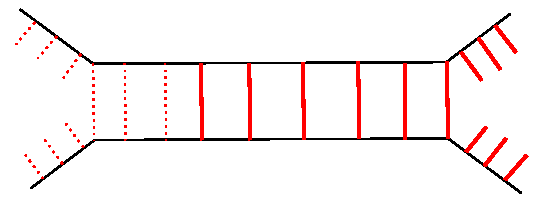
\includegraphics[width=0.6\textwidth]{./img/1__2.pdf}
\caption{\label{fig:9_1} Sequential unzipping from the ends.}
\end{figure}

\begin{figure}[h!]
\centering
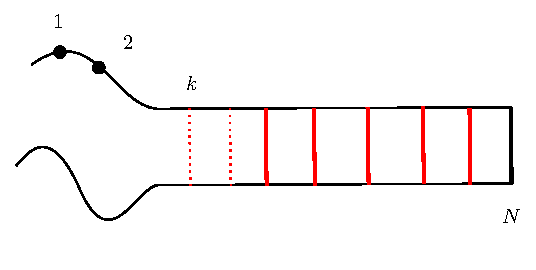
\includegraphics[width=0.6\textwidth]{./img/2__2.pdf}
\caption{\label{fig:9_2} Open and closed links in a single-ended zipper.}
\end{figure}

In this denaturation transition we do not allow bubbles.
Let us consider first the single-ended zipper, i.e. a molecular zipper of \emph{N} parallel links that can be opened only from one end as in Figure \ref{fig:9_2}. The single-ended zipper is simpler than any related problem which has been treated, and it offers a good way to introduce a biophysics example into a course of statistical mechanics.

If the first \emph{k} bonds (or links) are open (unbounded pairs) the energy to open the \emph{k+1} is \( \varepsilon _0 \). Note that if at least one of the previous \emph{k} bond is closed the energy needed to open the \( k+1 \) band is infinite! 
We specify further that the last link, \(k=N\), cannot be opened; this minor features serves only to distinguish one end from the other, and we shall say that the zipper is open when \(N-1\) links are open. 

We suppose that there are \emph{G} orientations which each open link can assume: that is, the open state of a link is \emph{G}-fold degenerate, corresponding to the rotational freedom of a link. Hence, once a bond is open it can orient itself in \emph{G} different ways. In other words, there is an entropy
\begin{equation}
  S_0 = k_B \log{G}
\end{equation}
associated to each open band. 
In the problem of DNA the empirical value of \emph{G} may be of the order of \(10^4\).

\subsubsection{Partition function}
Let us suppose that the energy required to open the first \emph{k} links is \(\varepsilon_0\). If \emph{k} links are open, the degeneracy is \(G^k\), and the contribution of this configuration to the partition function is 
\begin{equation*}
  G^k e^{-k \varepsilon _0/k_B T}
\end{equation*}
By summing over the possible values of \emph{k}, the partition function is
\begin{equation}
  Z_N (T,G, \varepsilon _0) = \sum_{k=0}^{N-1}  G^k e^{-k \varepsilon _0/k_B T} = \sum_{k=0}^{N-1} e^{k(S_0 T - \varepsilon _0)/k_B T}
\end{equation}
Let us call
\begin{equation}
  \chi \equiv G e^{-\varepsilon _0/k_B T}
\end{equation}
and simplify the previous expression
\begin{equation}
  Z_N = \sum_{k=0}^{N-1} \chi ^k = \frac{1-\chi^N}{1-\chi}
\end{equation}
We see immediately there is a single pole singularity.

The free energy is
\begin{equation}
  F_N = -k_B T \ln{Z_N} = -k_B T \ln{\qty[\frac{1-\chi^N}{1-\chi}]}
\end{equation}
We can now compute some observables of interest.
The correct procedure is to evaluate thermodynamic quantities for finite \(N\) and then to examine the limit \( N \rightarrow \infty\).

\subsubsection{Calculate average number of open links}
The thermodynamic average number of open links is
\begin{equation}
  \expval{k}_N \equiv  \frac{\sum_{k=0}^{N-1} k \chi^k}{\sum_{k=0}^{N-1} \chi^k } = \chi \dv[]{}{\chi} \ln{Z_N}  = \frac{N \chi^N}{\chi^N-1} - \frac{\chi}{\chi-1}
\end{equation}
The function is plotted in Figure \ref{fig:9_3}. We examine the behaviour of \( \expval{k}_N \)in the vicinity of the point \( \chi_c = 1 \) for which the denominators are equal to zero (pole).
\begin{remark}
In this model, we consider the average number of open links instead of the magnetization.
\end{remark}

\begin{figure}[h!]
\centering
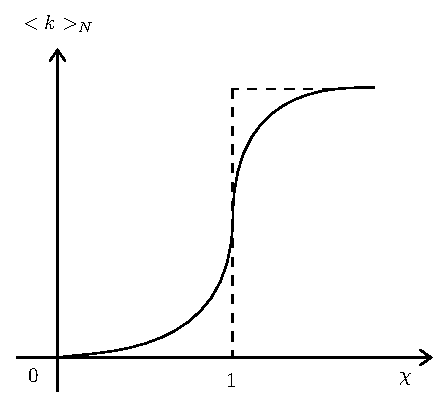
\includegraphics[width=0.4\textwidth]{./img/3__2.pdf}
\caption{\label{fig:9_3} Thermodynamic average number of open links in a single-ended zipper of \(N\) links.}
\end{figure}

 In order to analyze what happens near 1, we expand \( \chi \equiv 1+\varepsilon  \):

\begin{equation}
\begin{split}
  \log{Z_N} (\chi)  &=  \log{\qty[\frac{1-(1+\varepsilon )^N}{1-(1+\varepsilon )}] }  \\
  & =   \log{\qty[\frac{1-(1+\varepsilon N  + \frac{N(N-1)}{2!}\varepsilon ^2 + \frac{N(N-1)(N-2)}{3!}\varepsilon ^3 +O(\varepsilon ^4))}{\varepsilon }] } \\
  & = \log{\qty[N + \frac{N(N-1)}{2}\varepsilon + \frac{N(N-1)(N-2)}{6}\varepsilon^2 + \dots]  } \\
  & = \log{N} + \log{\qty[1+\frac{N-1}{2}\varepsilon +\frac{(N-1)(N-2)}{6}\varepsilon ^2] } \\
  & = \log{N} + \log{\qty[1+ \frac{N \varepsilon }{2}+ \frac{N^2 \varepsilon ^2}{6}+ \dots] }  \\
  & = \log{N} + \qty( \frac{N \varepsilon }{2} + \frac{N^2 \varepsilon ^2}{6} + \dots) + \frac{1}{2} \qty(\frac{N \varepsilon }{2} + \frac{N^2 \varepsilon ^2}{6} + \dots)^2  + \dots  \\
  & = \log{N}+ \frac{N \varepsilon }{2} + \frac{N^2 \varepsilon ^2}{24} + \dots
\end{split}
\end{equation}
By doing the same for \(   \expval{k}_N = \frac{N \chi^N}{\chi^N-1} - \frac{\chi}{\chi-1} \), one gets
\begin{equation}
  \expval{k}_N = \frac{N}{2} \qty( 1 + \frac{N \varepsilon }{6} - \frac{N^3 \varepsilon ^3}{360} + \dots)
\end{equation}
this is true for \( N \gg 1, \varepsilon \ll 1 \).

At the transition point \( \chi _c =1 \), where \( \varepsilon =0 \):
\begin{equation*}
  \expval{k}_N \simeq \frac{N}{2}
\end{equation*}
We can define the variation (slope per site) as a response function (the derivative with respect to the parameter):
\begin{equation}
  \frac{1}{N}\dv{\expval{k} }{\varepsilon } \simeq \frac{N}{12} - \frac{N^3 \varepsilon ^3}{240} + \dots
\end{equation}
is a maximum at \( \varepsilon =0 \), and the slope at the transition point becomes infinite as \( N \rightarrow \infty  \) (linearly). The response function diverges linearly to \emph{N}, this is a good signal that we have a transition.

\subsubsection{Transition temperature}
The temperature \( T_c \) corresponding to the pole \( \chi_c =1 \) is given by 
  \begin{equation*}
    G e^{-\varepsilon _0 /k_B T_c}  = 1
  \end{equation*}
Hence,
\begin{equation}
  T_c = \frac{\varepsilon _0}{k_B \log{G} }
  \label{eq:9_3}
\end{equation}
Note that as \( G \rightarrow 1 \), \( T_c \rightarrow 0 \). For \( G=1 \) there is no solution at a finite temperature and hence the model does not display a phase transition for any finite \emph{T}! This is telling you that if \( G=1 \) what is important it is the energy, you have no entropy as disorder. At that point everything can happen.

There is a finite transition temperature if \(G>1\). One might perhaps argue that the model is now not strictly one-dimensional, for the degeneracy \emph{G} arises from the rotational freedom of an open link.
\begin{remark}
Despite the model is 1-dim, for \( G>1 \) there is a phase transition. This is due to two contributions:
\begin{enumerate}
\item Existence of forbidden configuration (infinite energy). It is a necessary condition, but not sufficient, for a phase transition in \( d=1 \) with finite range interactions.
\item A further requirement may be that the degeneracy of the excited state (\emph{G}) of a structural unit must be higher than the degeneracy of the ground state\footnote{In the mean-field approximation no transition can occur if the degeneracy of the ground state is higher than that of the excited state.}.
\end{enumerate}
\end{remark}
\subsubsection{Unwinding from both ends}
When the zipper is allowed to unwind from both ends, there are \(k+1\) ways in which a total of \(k\) links may be opened, so that the partition function for a double-ended zipper of \(N\) links is
\begin{equation}
  Z_N (T,G, \varepsilon _0) = \sum_{k=0}^{N-1}  (k+1) G^k e^{-k \varepsilon _0/k_B T} 
\end{equation}
and to this should be added a term for the state of \(N\) open links. This terminal term for a simple zipper is \( G^N \exp(-N \varepsilon_0/ k_B T) \).

\subsection{Transfer matrix method for the Zipper model}
The idea is: we want to map the Zipper model to an Ising model. The spin like model consists on associating to each bond a spin such that \( S_i = 0 \) if the \emph{i}-esim bond is \emph{closed} , while \( S_i = 1, \dots, G \) if the \emph{i}-esim bond is \emph{open} with \emph{G} possible orientations. Therefore,
\begin{itemize}
  \item Case: \( S_i \neq 0 \) open. We have two subcases:
  \begin{itemize}
  \item \( S_{i-1}\) open: \( S_{i-1} \neq 0 \Rightarrow E (S_i \neq 0 | S_{i-1} \neq 0) = \varepsilon _0\).
  \item \( S_{i-1}\) closed: \( S_{i-1} = 0 \Rightarrow  E (S_i \neq 0 | S_{i-1} = 0) = \varepsilon _0 + V_0 \)
  \end{itemize}
\item Case: \( S_i = 0 \) closed. We have \( E (S_i=0)=0 \) irrespective of \( S_{i-1} \).
\end{itemize}
Hence, considering all these cases, the energy results
\begin{equation}
  E ( S_i, S_{i-1}) = ( \varepsilon _0 + V_0 \delta _{S_{i-1},0}) (1- \delta _{S_i,0})
\end{equation}
The boundary condition is \( S_N =0 \) (always closed).
The full Hamiltonian of the model can be written as (it could be also a function of delta, but it is not a problem):
\begin{equation}
  \mathcal{H}_N = \varepsilon _0 (1- \delta _{S_1,0}) + \sum_{i=2}^{N-1} (\varepsilon _0 + V_0 \delta _{S_{i-1},0})(1- \delta _{S_i,0})
\end{equation}
The Kittel's version is obtained by assuming \( V_0 = \infty  \).

The partition function is
\begin{equation*}
  Z_N = \sum_{\{ S \}  }^{} \exp (-\beta \mathcal{H}_N)
\end{equation*}
In order to implement the transfer matrix formalism we rewrite \( Z_N \) as follows
\begin{equation}
  Z_N = \sum_{\{ S \}  }^{} e^{-\beta \varepsilon _0 (1- \delta _{S_1,0})}  \prod_{i=1}^{N-2} e^{-\beta \varepsilon _0 (1- \delta _{S_{i+1},0}) }  \qty[1 + (e^{-\beta V_0}-1 ) \delta _{S_i,0}(1- \delta _{S_{i+1},0})] 
\end{equation}
Let us consider the Kittel model, the condition \( V_0 = \infty  \) implies \( \exp (-\beta V_0) = 0  \). Hence, we can define the transfer matrix as
\begin{equation}
  \mathbb{T} = \{ \bra{S} \mathbb{T} \ket{S'} \equiv t_{S,S'}   \}
\end{equation}
where
\begin{equation}
t_{S,S'} = e^{-\beta \varepsilon _0 (1- \delta _{S',0})} [1 - \delta _{S,0} (1- \delta _{S',0})]
\end{equation}
or in matrix form
\begin{equation*}
  \mathbb{T} =
  \begin{bmatrix}
    1 & 0 & \dots \dots 0 \\
    1 & a & \dots \dots a \\
    \vdots & \vdots   & \vdots \\
        \vdots & \vdots &  \vdots \\
        1 & a & \dots \dots  a
  \end{bmatrix},
  \qquad \text{with } a \equiv e^{-\beta \varepsilon _0}
\end{equation*}
The first think to notice is that the constraint that the bond \( S_{i+1} \) cannot be open if bond \( S_i \) is closed (\( S_i =0 \)) yields the null entries in the first row of \( \mathbb{T} \). This violates the hypothesis of the Perron-Frobenius theorem!

The matrix \( \mathbb{T} \) has three different eigenvalues
\begin{equation}
  \lambda _1 = Ga, \quad \lambda _2 =1, \quad \lambda _3 = 0
\end{equation}
The partition function can be written as
\begin{equation}
  Z_N = (1,a, \dots,a) \mathbb{T}^{N-2} \begin{pmatrix}
  1 \\
  1 \\
  \vdots \\
  1
  \end{pmatrix}
\end{equation}
Moreover, we have 
\begin{equation*}
  \lambda _1 \rightarrow \va{v}_1 = \begin{pmatrix}
  0 \\
  1 \\
  \vdots \\
  1
  \end{pmatrix},
  \qquad
  \lambda _2 \rightarrow \va{v}_2 = \begin{pmatrix}
  1-Ga \\
  1 \\
  \vdots \\
  1
  \end{pmatrix}
\end{equation*}
and we can then write
\begin{subequations}
\begin{align*}
  \begin{pmatrix}
  1 \\
  a \\
  \vdots \\
  a
\end{pmatrix}  &= \frac{a(1-Ga)-1}{1-Ga} \va{v}_1 + \frac{1}{1-Ga}\va{v}_2 \\
\begin{pmatrix}
1 \\
1 \\
\vdots \\
1
\end{pmatrix}  &= \frac{-Ga}{1-Ga} \va{v}_1 + \frac{1}{1-Ga}\va{v}_2
\end{align*}
\end{subequations}
Therefore,
\begin{equation}
  Z_N = \frac{1-(Ga)^N}{1-Ga} = \frac{1-(G e^{-\beta \varepsilon _0} )^N}{1-G e^{-\beta \varepsilon _0} }
  = \frac{1}{1-G e^{-\beta \varepsilon _0} } (-\lambda _1^N + \lambda _2^N)
\end{equation}

Since in the thermodynamic limit only the contribution of the largest eigenvalue matters for \( f_b \) we have
\begin{equation*}
  f_b = - k_B T \ln{\text{max} (\lambda _1, \lambda _2)}
\end{equation*}
\begin{remark}
Given that the \( \lambda _1 \) and \( \lambda _2 \) are positive, analytic function of \emph{T} (\( \lambda _1 = Ga, \lambda _2=1 \)). In order to have a phase transition
(i.e. non analiticity of \( f_b \)) the two eigenvalues must cross for a given value of \emph{T}. It is true if and only if:
\begin{equation}
  G a_c =1 \Leftrightarrow G e^{-\beta _c \varepsilon _0} = 1  \Leftrightarrow T_c = \frac{\varepsilon _0}{k_B \ln{G} }
\end{equation}
that agree with previous calculation (see Eq.\eqref{eq:9_3}).
\end{remark}


\section{Transfer matrix for \(\pmb{2-dim}\) Ising}
%The bibliography of this section is  \cite{9_lesson_1},\cite{9_lesson_2},\cite{9_lesson_3}.
The two-dimensional Ising model for a system of interacting spins on a square lattice is one of the very few nontrivial many-body problems that is exactly soluble and shows a phase transition \cite{9_lesson_2}. 
The exact solution in the absence of an external magnetic field (\(H=0\)) was first given almost eighty years ago in a famous paper by Onsager \cite{9_lesson_1}, using the theory of Lie algebras. In particular, from Onsager's solution we can see that already in two dimensions an Ising model can exhibit phase transitions, showing a non null spontaneous magnetization for temperatures low enough.

%Dimensional reducation from \emph{d} to \emph{d-1}. You can do the same for the 3D Ising model. In order to go smoothly to the one dimensional to the two dimensional the idea is to solve the Ising model to surfaces.

Let us therefore consider a two-dimensional Ising model, defined on a lattice made of \emph{N} rows and \emph{M} columns, as in Figure \ref{fig:9_4}. We apply periodic boundary conditions to the system in both directions (geometrically, this can be thought of as defining the model on a torus), and we  consider only nearest neighbour interactions.
The spin in a site is identified by \( S_{\text{site}} = S_{m,n} \).

\begin{figure}[h!]
\centering
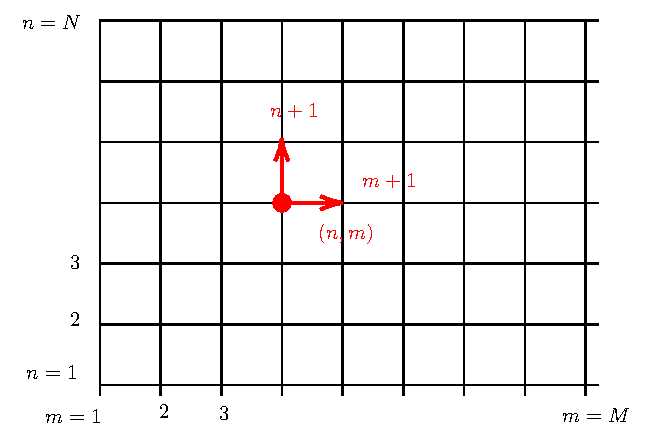
\includegraphics[width=0.6\textwidth]{./img/4__2.pdf}
\caption{\label{fig:9_4} 2-dimensional Ising lattice of \(N\) rows and \(M\) columns.}
\end{figure}

We consider a set of spin arranged on a square lattice, interacting only with nearest neighbors and with a magnetic field \(H  \neq 0 \).  The reduced Hamiltonian of the system will be:
\begin{equation*}
\begin{split}
  -\beta \mathcal{H}_ \Omega  ( \{ S \}  ) &= K \sum_{\expval{ij} }^{} S_i S_j + h \sum_{i}^{} S_i  \\
  & = K \sum_{n=1}^{N} \sum_{m=1}^{M} (S_{m,n} S_{m+1,n}+S_{m,n}S_{m,n+1}) + h \sum_{n=1}^{N} \sum_{m=1}^{M} S_{m,n}
\end{split}
\end{equation*}
This can be rewritten as follows:
\begin{equation}
  -\beta \mathcal{H}_ \Omega  ( \{ S \}  ) = \sum_{m=1}^{M} \qty[E_2(\mu _m, \mu _{m+1}) + E_1(\mu _m)]
\end{equation}
where 
\begin{subequations}
\begin{align}
E_1 (\mu _m,h) &= K \sum_{n=1}^{N} S_{m,n} S_{m,n+1} + h \sum_{n=1}^{N} S_{m,n} \\
  E_2 (\mu _m, \mu _{m+1},h) & = K \sum_{n=1}^{N} S_{m,n} S_{m+1,n}
\end{align}
\end{subequations}
the first equation is the one body interaction, while the second equation represents the interaction between nearest neighbours columns (two body interaction).

Moreover, \( \mu  \)  is a \emph{N} dimensional vector; in particular, each \( \mu _m \) represents the set of \emph{N} spins along column \emph{m}:
\begin{equation}
  \mu _m = \{ S_{m,1}, S_{m,2}, \dots, S_{m,N} \}
  \label{eq:9_1}
\end{equation}

We can write a transfer matrix between columns, permitting to transfer along the \emph{m}. As for the \( d=1 \) case we can make the Hamiltonian symmetric:
\begin{equation}
  -\beta \mathcal{H}_ \Omega  ( \{ S \}  ) = \sum_{m=1}^{M} \qty[E_2(\mu _m, \mu _{m+1}) + \frac{1}{2}(E_1(\mu _m) + E_1(\mu _{m+1}))]
\end{equation}

We have

\begin{equation}
\begin{split}
Z_{N,M}  &= \sum_{\mu_1}^{} \dots \sum_{\mu_M}^{} \exp \qty[ \sum_{m=1}^{M} \qty[E_2(\mu _m, \mu _{m+1}) + \frac{1}{2}(E_1(\mu _m) + E_1(\mu _{m+1}))]] \\
&= \sum_{\mu_1}^{} \dots \sum_{\mu_M}^{}  \qty[ \prod_{m=1}^{M} \exp  \qty[E_2(\mu _m, \mu _{m+1}) + \frac{1}{2}(E_1(\mu _m) + E_1(\mu _{m+1}))]] \\
& =  \sum_{\mu_1}^{} \dots \sum_{\mu_M}^{} \bra{\mu_1} \mathbb{T} \ket{\mu_2} \bra{\mu_2}  \mathbb{T} \ket{\mu_3} \dots \bra{\mu_N}  \mathbb{T} \ket{\mu_1}
\end{split}
\end{equation}

where

\begin{equation}
  \bra{\mu _m} \mathbb{T} \ket{\mu _{m+1}} = \exp \qty[E_2(\mu _m, \mu _{m+1}) + \frac{1}{2}(E_1(\mu _m) + E_1(\mu _{m+1}))]
  \label{eq:9_2}
\end{equation}


\begin{remark}
In the 2x2 transfer matrix in the 1-dim case we have two possible values. Now, we have to do the same in principle, but we have to do for all of the \eqref{eq:9_1}.
\end{remark}
\begin{remark}
\( \mathbb{T} \) is a matrix of dimension \( 2^N \times 2^N \), hence, in the thermodynamic limit is an infinite matrix (violation of Perron-Frobenius).
\end{remark}




 If we can find the set of eigenvalues \( \lambda _+ > \lambda _- \ge \lambda _1 \ge \dots \ge \lambda _{2^N-2} \) of the  \( 2^N \times 2^N \) matrix, we have

\begin{equation}
      Z_{N,M}  = \Tr(\mathbb{T}^M) = \sum_{i= \pm, 1}^{ 2^N-2} \lambda _i^{M}(N)
\end{equation}

%%%%%%%%%%%%%


\subsubsection*{Thermodynamic Limit}
We can write our bulk free-energy as:
$$\begin{align}
f_{b} &= -k_{B}T \lim_{ N \to \infty } \lim_{ M \to \infty } \frac{1}{MN} \ln(Z) \\
&= -k_{B}T \lim_{ N \to \infty } \lim_{ M \to \infty } \frac{1}{NM} \ln(\lambda_{+}^{M} + \lambda_{-}^{M} + \dots) \\
&= -k_{B}T \lim_{ N \to \infty } \frac{1}{N}\ln(\lambda_{+}) - k_{B}T \lim_{ N \to \infty } \lim_{ M \to \infty } \frac{1}{MN} \ln\left[ 1 + \sum_{k} \left( \frac{\lambda_{k}}{\lambda_{+}} \right)^{M} \right]  \\
&= -k_{B}T \lim_{ N \to \infty } \frac{1}{N}\ln(\lambda_{+})(N) \quad (\star)
\end{align}$$
Our ultimate goal is to find the largest eigenvalue of the $2^{N}\times 2^{N}$ matrix and take the limit $(\star)$.
Not an easy task to achieve.
The first solution was given by ONSAGER using Lie Algebra and group representation for $H = 0$ (1944).
Subsequent alternative method include Pfaffian or other combinatorial methods or mapping to a $1d$ quantum mechanics system.
Let us jump directly to the final result:
$$\lambda_{+}(N) = \left[ 2 \frac{\sinh}{2k} \right]^{\frac{N}{2}} \exp\left[ \frac{1}{2}\sum_{i=1}^{2N -1}\psi_{i} \right]$$
where $\psi_{i}$ are defined such that:
$$\cosh(\psi_{i}) = \coth(2k)\cosh(2k)-\cos\left( \frac{i\pi}{N} \right)$$
So we can write our bulk free-energy as:
$$f_{b} = -k_{B}T\lim_{ N \to \infty } \ln(\lambda_{+}) = -\frac{k_{B}T}{2}\ln[2\sinh(2k)] - k_{B}T \lim_{ N \to \infty } \frac{1}{2N}\sum_{i=1}^{N}\psi_{2i - 1}$$
In the thermodynamic limit ($N\to \infty$):
$$\frac{1}{2N} \sum_{i=1}^{N} \psi_{2i-1} \sim \frac{1}{2\pi} \int _{0}^{\pi} \psi(\theta) \, d\theta = \frac{1}{2\pi} \int _{0}^{\pi}\text{arccosh}[\coth(2k)\cosh(2k) - \cos(\theta)] \, d\theta $$
using the identity
$$\text{arcosh}(x) = \frac{1}{\pi} \int _{0}^{\pi}\ln[2(x-\cos(\phi))] \, d\phi $$
we can write finally
$$f_{b} = -\frac{k_{B}T}{2} \ln[2\sinh(2k)] - \frac{k_{B}T}{2}\ln 2 - \frac{k_{B}T}{2\pi^{2}} \int _{0}^{\pi}\int _{0}^{\pi} \ln[\coth(2k)\cosh(2k) - \cos(\theta) - \cos(\phi)] \, d\phi  \, d\theta $$
From the expression $f_{b}$ one can deduce all the thermodynamic properties of the $2D$ Ising Model for $H = 0$.
Where the expression from which derive  \(T_c\) is:
\begin{equation*}
  2 \tanh^2 \qty(\frac{2J}{k_B T_c}) = 1 
\end{equation*}
 which yields the numeric result:
 \begin{equation*} \Rightarrow T_c \simeq 2,264 J/k_B \neq 0
\end{equation*}
hence, we have a phase transition at a critical temperature \(T_c\) different from 0!
Onsager also showed that the critical exponents of this model are:
\begin{equation*}
\alpha =0,\quad \beta=\frac{1}{8}, \quad \gamma = \frac{7}{4}
\end{equation*}
where \(\alpha=0\)  because the specific heat diverges logarithmically for \(T \sim T_c\):
\begin{equation*}
  c \propto A \qty[-\ln{\qty(1- \frac{T}{T_c}) } + B  ]
\end{equation*}
It means that the specific heat displays at the transition a logarithmic divergence (no power law!).






\end{document}
